% The third chapter about the code's conzept
% @author Kalvin Döge
%


\chapter{Konzept}\label{ch:konzept}

Im Folgenden wird das Model der Simulation konzeptioniert und ausgeführt, mit den vorherigen Begriffserklärungen als Grundlage.
Dabei wird auf den Simulationsort im Modell, den Aufbau und Voreinstellungen der Agenten und Lichtsignalschaltungen, die Projektarchitektur und zuletzt noch auf den Umfang der Arbeit eingegangen.

% The section about the simulation's type
% @author Kalvin Döge
%


\section{Simulationstyp}\label{sec:simulationtype}

Für diese Arbeit empfiehlt sich eine agentenbasierte Simulation, da im Vornherein die zu fahrende Route eines Agenten zwar bekannt ist, die Einflüsse von zum Beispiel Pkws aber direkt im Übergang von einer Lichtsignalschaltung zur anderen den Akteur beeinflussen und so nicht vorhergesehen werden können.
Damit also keine Annahmen über dynamische, umwelt- oder agentenbedingte Einflüsse im Quellcode festgelegt werden, ist entsprechend eine agentenbasierte Echtzeitsimulation angemessener für diese Simulation.

% The section about the place of the simulation itself
% @author Kalvin Döge
%


\section{Simulationsort}\label{sec:simulationplace}

Für die Arbeit wurde die Binnen- und Außenalster als Simulationsumgebung ausgewählt.

\begin{figure}[h]
    \centering
    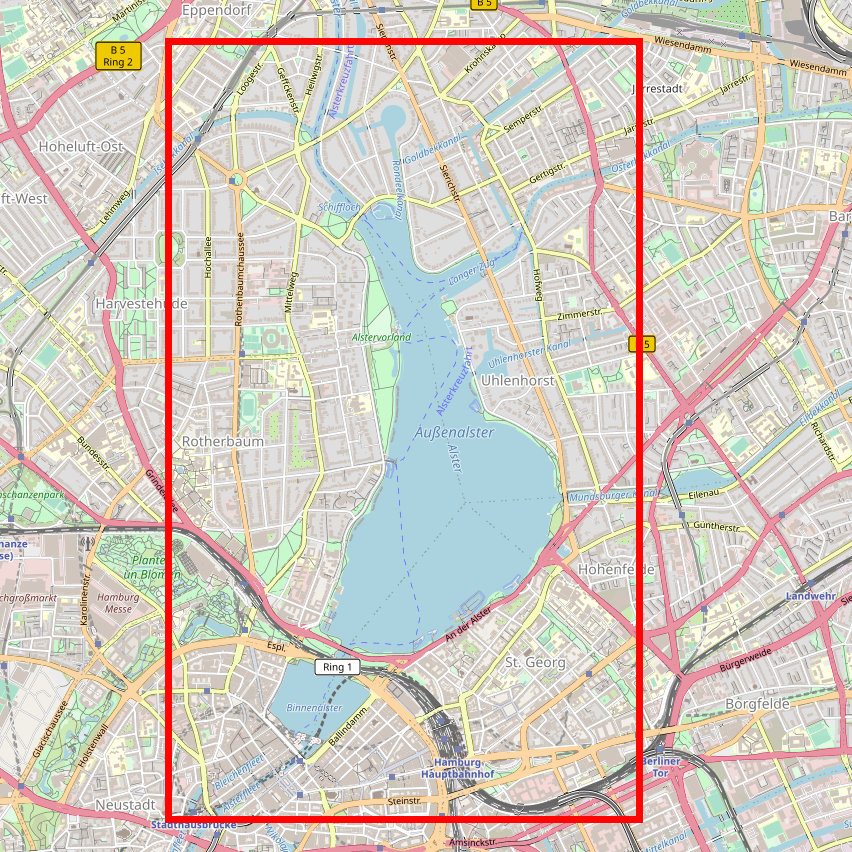
\includegraphics[width=0.75\textwidth]{sim-area}
    \caption{Simulationsumgebung}
    \label{fig:sim-area}
\end{figure}

Wie im Ausschnitt~\ref{fig:sim-area} zu erkennen ist, ist aufgrund der zentralen Lage innerhalb der Stadt, vieler anliegenden Kreuzungen und generell dichter Besiedelung um die Alster herum eine hohe Dichte an Agenten für die Simulation gegeben, die eine ,,Grüne Welle`` für Fahrradfahrer erschweren können.
Dies gibt der Simulation auf der einen Seite eine Herausforderung, mit schwereren Vorgaben überhaupt eine Lichtsignalschaltung für die ,,Grüne Welle`` zu finden, während auf der anderen Seite dafür aber diese Simulation wie eine ,,Obergrenze`` angesehen werden kann für die Agenten- und Lichtsignalanzahlen.

% The section about the agents of the simulation itself
% @author Kalvin Döge
%


\section{Agenten}\label{sec:agents}

Im Folgenden werden die Konzepte der Agenten näher erläutert, wobei besonders auf die Grundlagen der Agenten, ihre Modalitäten, die Interaktion mit anderen Agenten und Entitäten, die Anzahl an aktiven Agenten und auf die gefahrene Routen eingegangen wird.

% The section about the agents' modalities of the simulation itself
% @author Kalvin Döge
%

\subsection{Voraussetzungen}\label{subsec:prerequisities}

Es gibt zwei Arten von Agenten, die in der Simulation agieren: Den Nebenagenten, fortan ,,\code{HumanTraveler}`` genannt, und dem Hauptagenten, fortan ,,\code{BicycleLeader}`` genannt.

Der \code{BicycleLeader} ist der Fokus dieser Arbeit.
Dieser wird immer mit einem eigenen Fahrrad oder einem mietbaren Fahrrad ausgestattet, mit dem er vorgegebene Punkte auf einer Route um die Alster abfahren soll.
Sein Ziel ist es, eine Runde um die Alster zu fahren, ohne dabei auf 0 km/h bremsen zu müssen.
Langsames Fahren ist hier nicht mit einbezogen als Fehlschlagbedingung, da eine Schwelle für ,,zu langsames`` Fahren, sodass der \code{BicycleLeader} sein Gleichgewicht nicht mehr halten könne, von einer Reihe von Faktoren abhängt, die außerhalb des Rahmens dieser Arbeit wären: das Alter des BicycleLeaders, die Erfahrung mit dem Fahrrad, das angestrebte Fahrverhalten, Höhenprofile der Umgebung, Wetterbedingungen und noch einige Aspekte mehr.

\code{HumanTraveler} sind dabei die Einwohner, die mit Lichtsignalschaltungen interagieren und auf den Straßen dem \code{BicycleLeader} in die Quere kommen.
Das Ziel der \code{HumanTraveler} ist es lediglich, ein zufällig zugewiesenes Ziel um die Alster herum zu erreichen, bevor sie aus der Simulation entfernt werden.

% The section about the agents' modalities of the simulation itself
% @author Kalvin Döge
%

\subsection{Modalitäten}\label{subsec:modalitaten}

Die \code{HumanTraveler} haben drei Arten der Transportation zur Verfügung: zu Fuß, Pkws und Fahrräder.
In dem MARS-Framework ist es Agenten ebenso gestattet, bei Autos und Fahrrädern diese zu Mieten und damit sogenannte ,,RentalCars'' oder ,,RentalBikes'' zu nutzen, jedoch hat es für diese Arbeit keinen großen Einfluss, ob sie ihr eigenes Transportmittel nehmen oder einen Umweg zu den mietbaren Äquivalenten einschlagen, da die Agenten in der Simulation nur als ,,Störfaktor`` über Ampeln und auf Straßen mit dem Hauptagenten interagieren.

Für jede Modalität gibt es eine vorgesehene Straße zum Befahren: Pkws fahren auf Straßen, Fahrräder fahren auf Fahrradlinien und teilweise auch auf Straßen.
Fußgänger können sich nur auf Fußgängerwegen bewegen, dafür können sie in andere Modalitäten wechseln.
Jeder \code{HumanTraveler} als auch der \code{BicycleLeader} beginnt die Simulation als Fußgänger, bevor sie auf eine Modalität aufsteigen.

% The section about the agents' modalities of the simulation itself
% @author Kalvin Döge
%

\subsection{Interaktionen mit Agenten und Entitäten}\label{subsec:interactions}

Interaktionen zwischen Agenten sind in dieser Simulation beschränkt auf zwei Arten: dem Verlangsamen und Blockieren auf Straßen als auch dem Aufhalten von anderen Agenten an Lichtsignalschaltungen.
\code{HumanTraveler} und \code{BicycleLeader} können über ihre Pkws und Fahrräder an Ampeln einen Platz einnehmen und damit die Warteschlangen verlängern.
Je länger sie wird, desto mehr Zeit benötigt die Simulation, um die Warteschlange bei einem grünen Signal zu leeren.

Auf den Straßen und Fahrradwegen selbst haben die jeweiligen Modalitäten nur dann miteinander Interaktionen, wenn sie sich zu Nahe kommen.
Damit es nicht zu Kollisionen kommt, wird überprüft, wie nahe sich zwei Agenten sind, um dann zu verlangsamen oder weiterzufahren.
Eine detailliertere Abhandlung dazu wird im Kapitel ,,Implementierung`` angegangen.

% The section about the agents' amount of the simulation itself
% @author Kalvin Döge
%

% graphics

\subsection{Anzahl aktiver Agenten}\label{subsec:activeagents}

Zur Bestimmung von der Anzahl an aktiven Agenten, wurde eine angenäherte Rechnung für die Population um die Alster genommen, da direkte Statistiken zur täglichen Anzahl an Verkehrsteilnehmern in Hamburg beziehungsweise in verschiedenen Stadtvierteln fehlen.
Um eine Annäherung an die Verkehrszahlen zu bekommen, wird zuerst die Verteilung über Haupt-, Neben- und Schwachverkehrszeiten untersucht.

Ein Arbeitstag, Montag bis Freitag, hat zwei große Hauptverkehrszeiten: morgens von 6 bis 9 Uhr und nachmittags von 15 bis 19 Uhr~\cite{FHH2015}.
In diesen beiden Zeiten werden die meisten Verkehrsteilnehmer auf den Straßen unterwegs sein und damit am ehesten Staus verursachen.

Die Nebenverkehrszeit tritt von 9 bis 15 Uhr~\cite{FHH2015} auf, die den Übergang zwischen den beiden Hauptverkehrszeiten darstellt.
Innerhalb dieser Zeit ist die Dichte an Verkehrsteilnehmern geringer als in der Hauptverkehrszeit, aber immer noch höher als in Schwachverkehrszeiten.

Die Schwachverkehrszeit ist von 20 Uhr bis 5 Uhr am nächsten Tag~\cite{FHH2015}, in der der Verkehr am geringsten ist, die Straßen leer und der Stau am seltensten auftritt.


Um den Verlauf über einen Tag nun mit zwei Hochpunkten und drei Tiefpunkten darzustellen, während dabei der zweite Tiefpunkt höher als der erste und dritte ist, könnte man eine negierte Funktion 4.\ Grades benutzen.

\begin{figure}[h]
    \centering
    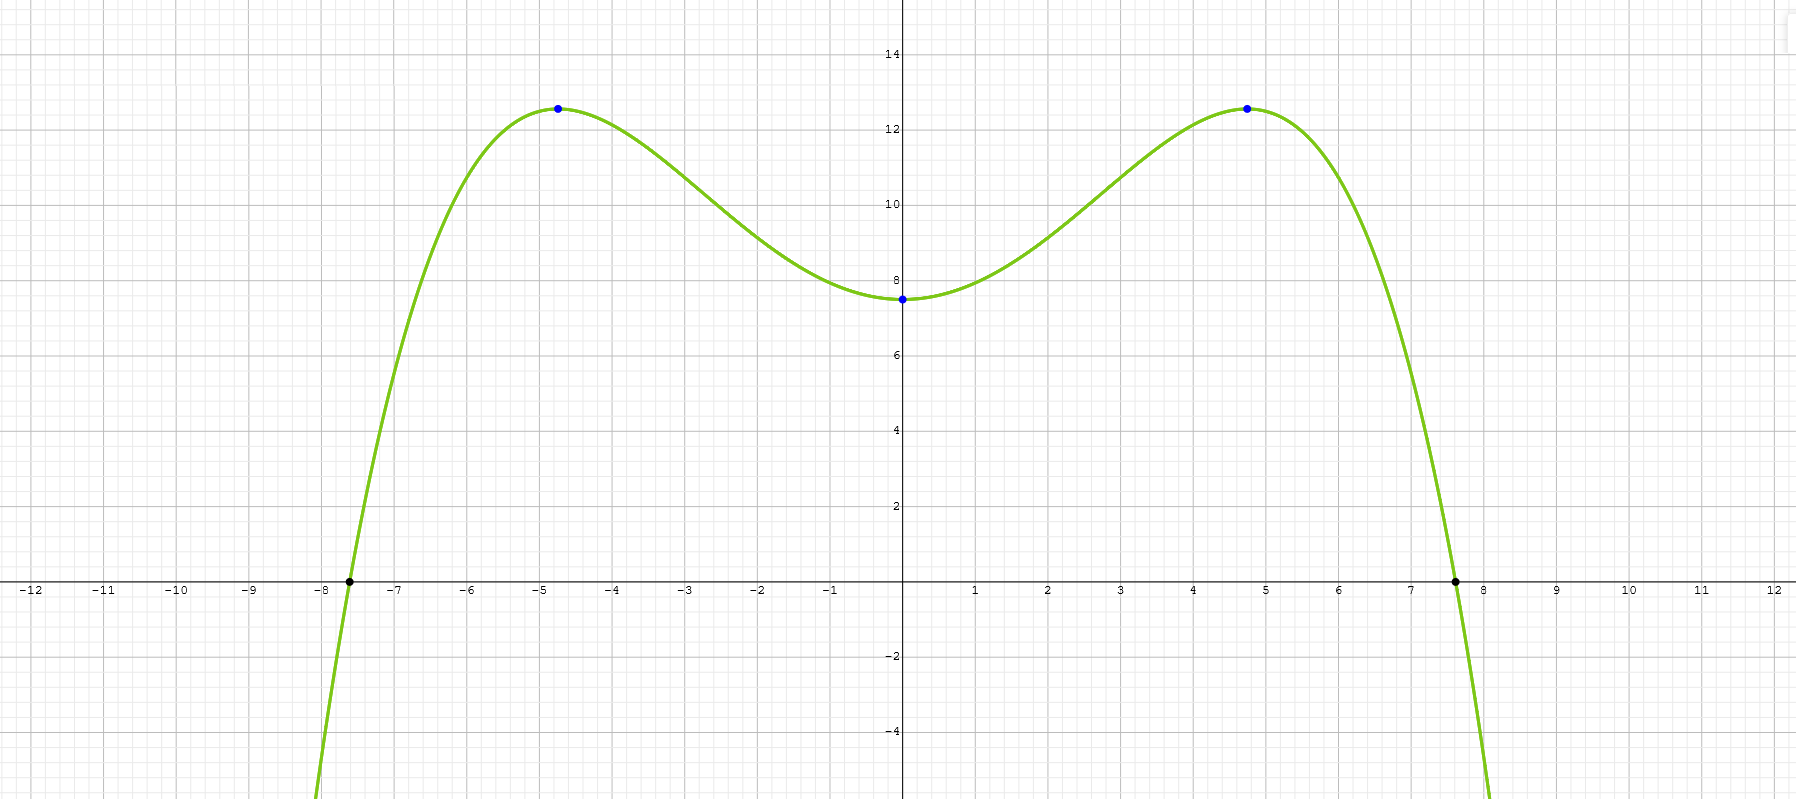
\includegraphics[width=1.00\textwidth]{poly-4-degree}
    \caption{Polynomialfunktion des 4. Grades zur Annäherung}
    \label{fig:poly-4-degree}
\end{figure}

Die Funktion aus der Grafik~\ref{fig:poly-4-degree} lautet: \[f(x)=-0.01x^4+0.45x^2+7.5\]

Die Grafik~\ref{fig:poly-4-degree} muss so interpretiert werden, als hätte die x-Achse eine Verschiebung von 12 Einheiten nach rechts noch erhalten, damit die Werte sich passend der Tagesstunden verteilen.
Entsprechend ist 0 Uhr hier bei x = -12, 12 Uhr ist bei x = 0 und 24 Uhr ist bei x = 12.

Zum Annähern selbst ist die Funktion aber nur ansatzweise nützlich, da wenn x die Stundenanzahl und f(x) der Prozentsatz aller aktiven Agenten darstellt, die Schwachverkehrszeiten bei einer Funktion 4.\ Grades auf der x-Achse in das Negative gehen würden.
Damit wäre aber, wenn f(x) Nullstellen bei \[x = -12, x = 12\] hätte, keine relativ gleiche Verteilung über die 9 Stunden, also wäre von 20 bis 5 Uhr keine relativ flache Schwachverkehrszeit.
Der zweite Ansatz wäre, bei einem anderen x-Wert die Nullstelle schneiden zu lassen, wie es in der Grafik~\ref{fig:poly-4-degree} zu sehen ist, also zum Beispiel an den Stellen \[x = -7.6, x = 7.6\]
x = -7.6 wäre um circa 4 Uhr und x = 7.6 wäre um circa 20 Uhr.
Bei diesem Ansatz werden dann aber negative Funktionswerten außerhalb der x-Werte auftreten und damit ,,negativen Verkehr`` verursachen.
Das kann logischerweise nicht in der realen Welt auftreten, also müssen die Werte auf 0 oder einen anderen Wert gesetzt werden.
Sollte der Wert auf 0 gesetzt werden, wäre das noch immer keine korrekte Darstellung für das Modell, da in der Schwachverkehrszeit noch immer Verkehr vorliegt.
Um einen besseren Funktionsverlauf zu gewährleisten, muss die Funktion interpoliert werden, um flachere Übergänge in die Schwachverkehrszeit zu bewerkstelligen.
Um den Verlauf beziehungsweise die Interpolation zu konstruieren, werden kubische Polynome genutzt, die an bekannten Punkten eine Ober- beziehungsweise Untergrenze bilden und damit übergehen in die nächste, kubische Funktion.
Mithilfe Timo Denks Implementation der kubischen Spline-Interpolation~\cite{Denk2018} lässt sich mithilfe der Datenpunkte aus der Vorabinformation von der Stadt Hamburg annähern.


$f(x) = \begin{cases}
            8.8699 \cdot 10^{-2}\cdot x^3 -1.4163 \cdot 10^{-59}\cdot x^2 + 2.0171 \cdot 10^{-1}\cdot x + 0.0000, & \text{if } x \in [0,3], \\-2.0275 \cdot 10^{-1}\cdot x^3 + 2.6231\cdot x^2 -7.6675\cdot x + 7.8692, & \text{if } x \in (3,6], \\9.4824 \cdot 10^{-2}\cdot x^3 -2.7333\cdot x^2 + 2.4471 \cdot 10^{1}\cdot x -5.6408 \cdot 10^{1}, & \text{if } x \in (6,12], \\-8.5660 \cdot 10^{-2}\cdot x^3 + 3.7641\cdot x^2 -5.3498 \cdot 10^{1}\cdot x + 2.5547 \cdot 10^{2}, & \text{if } x \in (12,18], \\1.2958 \cdot 10^{-1}\cdot x^3 -7.8589\cdot x^2 + 1.5572 \cdot 10^{2}\cdot x -9.9981 \cdot 10^{2}, & \text{if } x \in (18,22], \\-1.1557 \cdot 10^{-1}\cdot x^3 + 8.3212\cdot x^2 -2.0025 \cdot 10^{2}\cdot x + 1.6106 \cdot 10^{3}, & \text{if } x \in (22,24].
            \label{fig:interpolation}
\end{cases}$

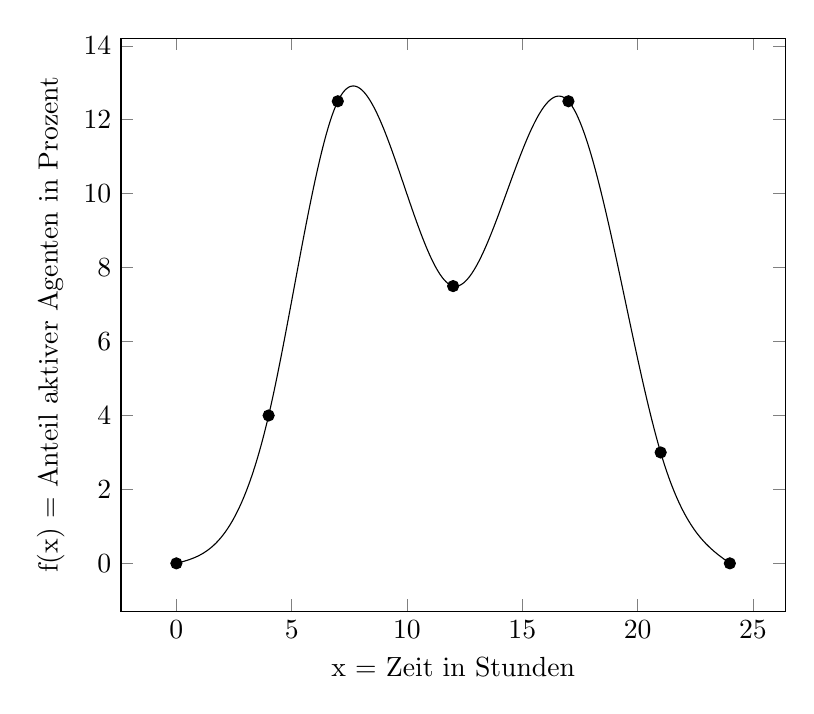
\begin{tikzpicture}
    \pgfplotsset{
        scale only axis,
    }

    \begin{axis}
        [
        xlabel={x = Zeit in Stunden},
        ylabel={f(x) = Anteil aktiver Agenten in Prozent},
        samples=100,
        ]
        \addplot [only marks] table {
            0 0
            4 4
            7 12.5
            12 7.5
            17 12.5
            21 3
            24 0
        };


        \addplot[][domain=0:4]{+0.05212125853316996*x^3+3.4e-60*x^2+0.1660598634692806*x^1+0*x^0};
        \addplot[][domain=4:7]{+-0.19010136076913603*x^3+2.9066714316276716*x^2+-11.460625863041406*x^1+15.502247635347583*x^0};
        \addplot[][domain=7:12]{+0.12557646303751677*x^3+-3.722562868312037*x^2+34.94401423653655*x^1+-92.77524593033432*x^0};
        \addplot[][domain=12:17]{+-0.11369945737791003*x^3+4.891370266643328*x^2+-68.42318338292783*x^1+320.6935445475232*x^0};
        \addplot[][domain=17:21]{+0.12176450638893752*x^3+-7.117291885465897*x^2+135.724073202929*x^1+-836.1409094389987*x^0};
        \addplot[][domain=21:24]{+-0.061541335226351856*x^3+4.430976136297334*x^2+-106.78955525409884*x^1+861.454489760196*x^0};
    \end{axis}
    \label{fig:interpolation-graph}
\end{tikzpicture}


Nun muss nur noch die Einwohnerdichte pro km\textsuperscript{2} angenähert werden, damit man eine grobe Gesamtanzahl an Agenten ableiten kann.
Das Statistikamt Nord, das für Schleswig-Holstein und Stadtteile Hamburgs Statistiken sammelt, hat in ihrem Bericht aus dem Jahr 2021 die Einwohnerdichte aller Stadtteile Hamburgs aufgelistet~\cite{SAHHSH2022}.
Der Simulationsort dieser Arbeit umfasst die folgenden Stadtteile: Neustadt, St. Georg, Hohenfelde, Uhlenhorst, Winterhude, Eppendorf, Harvestehude und Rotherbaum.
Für diese Stadtteile wird die Einwohnerdichte pro km\textsuperscript{2} ausgelesen:

\begin{center}
    \begin{tabular}{||c c c c||}
        \hline
        Stadtteil    & Einw.\ je km\textsuperscript{2} \\ [0.5ex]
        \hline\hline
        Neustadt     & 5575                            \\
        \hline
        St. Georg    & 6291                            \\
        \hline
        Hohenfelde   & 8578                            \\
        \hline
        Uhlenhorst   & 8516                            \\
        \hline
        Winterhude   & 7499                            \\
        \hline
        Eppendorf    & 9193                            \\
        \hline
        Harvestehude & 8636                            \\
        \hline
        Harvestehude & 6253                            \\
        \hline\hline
        Gesamt       & 60.541         \\[1ex]
        \hline
    \end{tabular}
\end{center}

Es werden absichtlich aus dieser Statistik manche Agentengruppen nicht entfernt oder hinzugefügt, da keine genauen Statistiken dazu von der Stadt Hamburg gegeben oder bei der Recherche aufgefunden werden konnten zum Verwenden in dieser Arbeit.
Jene Gruppen umfassen, sind aber nicht beschränkt auf: Kinder, Eltern, die Zuhause auf Kindern aufpassen, Home-Office-Workers, Alte oder kranke Leute, Arbeitslose und noch mehr.
Diese müssten theoretisch gesehen aus den Statistiken entfernt werden, während folgende Menschengruppen zu der Statistik hinzugezählt werden müssten: Pendler aus anderen Städten, Pendler aus anderen Stadtvierteln, Privatpersonen mit mehr als einem Fahrtziel, Berufsfahrer wie zum Beispiel Taxis oder Lieferanten, Touristen und so weiter.
Der Einfachheit halber wurde also die durchschnittliche Einwohnerzahl der betroffenen Stadtviertel genommen, anstatt alle Umweltfaktoren aus der echten Welt einzubeziehen.

Mit der Gesamtmenge an Einwohnern pro km\textsuperscript{2} lässt sich der Durchschnitt aller für dieser Simulation relevanter Stadtteile berechnen, der dann mit der Gesamtfläche des Simulationsortes multipliziert die Gesamtanzahl an aktiven Agenten ergibt.
Der Flächeninhalt der Simulation ist mithilfe einer OpenStreetMap-Karte~\cite{OSF2004} berechenbar:

\begin{figure}[h]
    \centering
    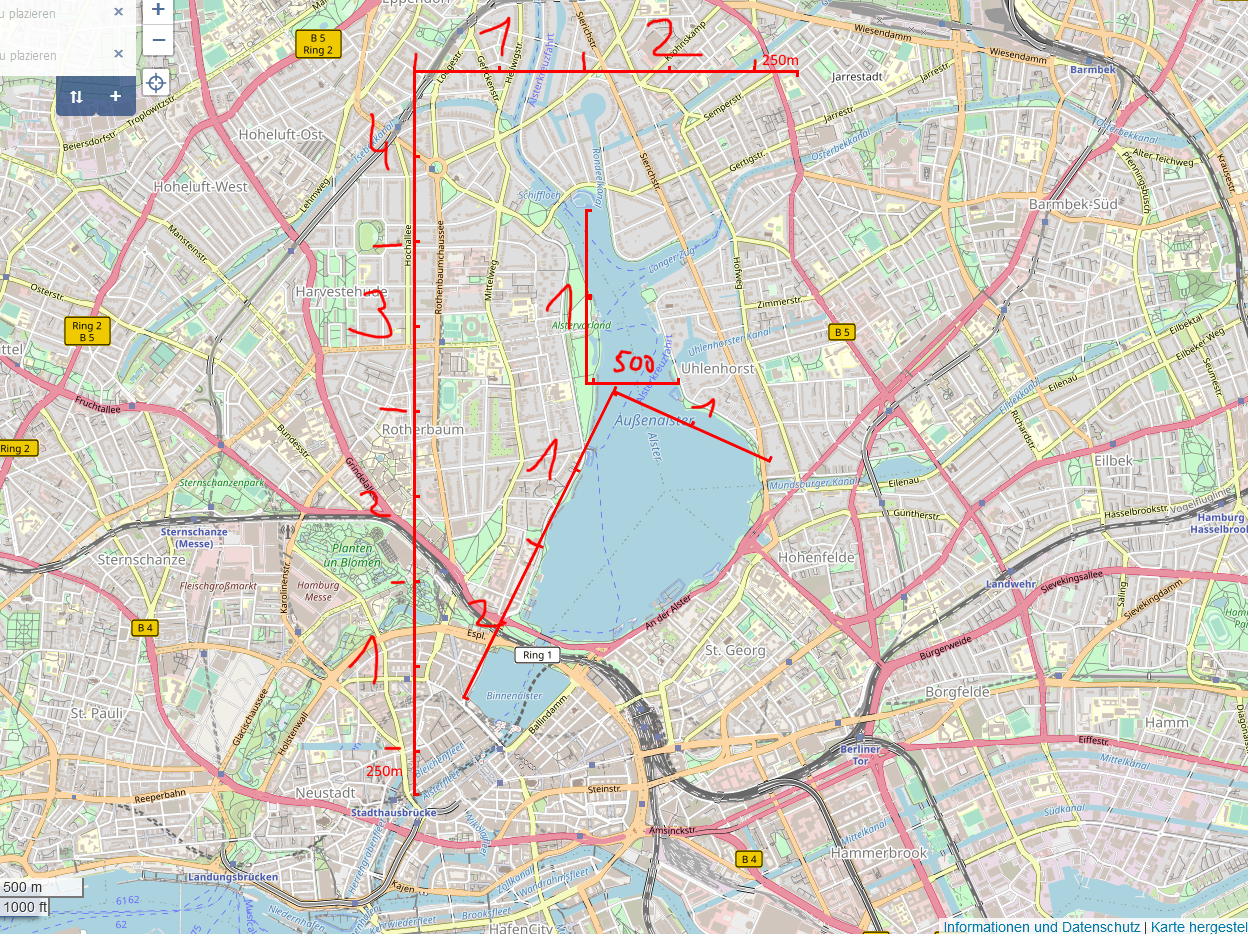
\includegraphics[width=0.75\textwidth]{calc-area}
    \caption{Grobe Flächenberechnung der bewohnbaren Bereiche}
    \label{fig:calc-area}
\end{figure}

Aus der Grafik~\ref{fig:calc-area} lassen sich folgende Flächen ablesen:

\begin{align}
    A &= (4,25~\unit{~km} * 2,25~\unit{~km}) - (0,5~\unit{~km}^2 + 2~\unit{~km}^2) \\
    &=  9,56~\unit{~km}^2 - 2,5~\unit{~km}^2 \\
    &=  7,06~\unit{~km}^2
\end{align}

Zuletzt wird noch die Multiplikation der durchschnittlichen Einwohnerdichte mit dem Flächeninhalt berechnet:

\begin{align}
    Gesamtanzahl Agenten &= 7,06~\unit{~km}^2 * ((60.541~\unit{~Einw~je~km}^2) / 8) \\
    &= 7,06~\unit{~km}^2 * (7.567,625~\unit{~Einw~je~km}^2) \\
    &= 53.427,4325~\unit{~Einw.~je~km}^2 \\
    &\approx 53.427~\unit{~Einw.~je~km}^2
\end{align}

Mit den Voraussetzungen lässt sich für jeden beliebigen Zeitpunkt an einem Arbeitstag eine Annäherung mit der Interpolationsgleichung~\ref{fig:interpolation} berechnen.
In der Simulation wird für jede Stunde, die neu angefangen wird, ein neuer Wert aus der Gleichung mit der durchschnittliche Einwohnerdichte multipliziert und damit als für diese Stunde, aktive Anzahl an Agenten festgelegt.
In dieser Simulation werden nur Daten für jede Stunde genommen, da der \code{BicycleLeader} ebenfalls nur jede Stunde einmal die Route fährt.

% The section about the agents' routes
% @author Kalvin Döge
%

\subsection{Agentenrouten}\label{subsec:routs}

In diesem Model haben \code{HumanTraveler} nur zwei Punkte auf ihrer Route, die sie erreichen müssen: Den Startpunkt, auf dem sie beginnen, und das Endziel, das ein beliebiger Punkt im Simulationsbereich ist.
Diese Agenten haben, wie bei dem Unterkapitel ,,Modalitäten`` bereits erwähnt, dafür drei verschiedene Transportarten zur Verfügung, und sind nicht weiter eingeschränkt in der Art und Weise, wie sie zum Zielpunkt gelangen.

\begin{figure}[h]
    \centering
    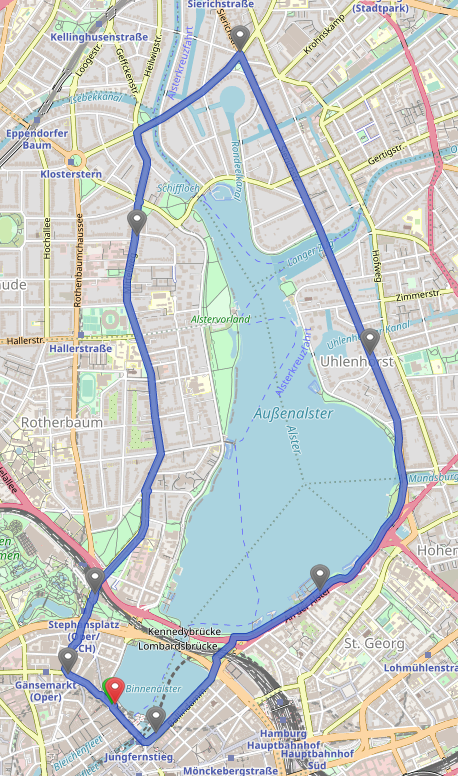
\includegraphics[width=1.00\textwidth]{route}
    \caption{Route der Bicycle-Leader mit den 8 Zwischenpunkten}
    \label{fig:bicycleleader-route}
\end{figure}

Der \code{BicycleLeader} wiederum, wie anhand der Grafik~\ref{fig:bicycleleader-route} zu entnehmen ist, hat 8 Punkte abzufahren, die um die Binnen- und Außenalster verteilt sind:
Die Route beginnt und endet bei dem Café Alex, während die restlichen 6 Punkte verteilt um die Alster platziert sind, damit eine Rundfahrt bei möglichst vielen Lichtsignalschaltungen geplant sind.



% The section about the agents of the simulation itself
% @author Kalvin Döge
%


\section{Lichtsignalschaltungen}\label{sec:lightsignals}

Die Lichtsignalschaltungen stellen die größte Barriere und der Fokus dieser Simulation: Ihre Aufgabe ist es, Pkws und Fahrräder aufzuhalten, wenn sie in der Rotphase sind und sie durchzulassen, wenn sie Grün sind.

% The section about the lightsignals' generel description
% @author Kalvin Döge
%

\subsection{Beschreibung der Lichtsignalanlagen}\label{subsec:description}

Während der Rotphase ist es möglich, dass sich mehrere Verkehrsteilnehmer an der Ampel anstauen und dadurch eine Warteschlange bilden, die sich erst bei Grün mit einer Geschwindigkeit von einem Verkehrsteilnehmer pro Sekunde leert.
Bei einer Warteschlange von 20 Leuten ist es also der letzten \code{HumanTraveler} erst möglich, die Ampel hinter sich zu lassen, sobald alle 19 Verkehrsteilnehmer vor dem \code{HumanTraveler} nach 19 Sekunden durchgelassen wurden.

Die Positionsdaten der Ampeln im Simulationsbereich sind mit dem OpenStreetMap-Tool cite{OSF2004} entnommen worden und dann für die Simulation aufbereitet in Form von \code{Longitude}- und \code{Langitude}-Werten.

% The inner workings of the light signals
% @author Kalvin Döge
%

\subsection{Funktionsweise von Lichtsignalschaltungen}\label{subsec:workings}

Die Funktionsweise der Lichtsignalschaltungen während der Simulation lässt sich in zwei Schritte zusammenfassen: 1.\ Timer fortsetzen und 2.\ die Warteschlange überprüfen.

Der Timer wird im ersten Schritt um eine Sekunde fortgesetzt.
Ist der aktuelle Timer-Wert über der Zeitgrenze von einer Rot-, Gelb- oder Grünphase, wird die Phase gewechselt.
Ist der Timer-Wert über die Summe von Rot-, Gelb- und Grünphasenlänge hinaus, setzt sich der Timer wieder zurück auf 1 verstrichene Sekunde.

Im zweiten Schritt wird die Warteschlange überprüft.
Ist der Verkehrsteilnehmer nicht mehr an dieser Ampel, weil der Teilnehmer der erste in der Schlange ist und die derzeitige Ampelphase Grün ist, so wird dieser aus der Warteschlange entfernt.
Das Wegfahren selbst unternimmt immer noch der Pkw-Fahrer selbst.

% The section about the lightsignals' phases
% @author Kalvin Döge
%


\subsection{Lichtsignalphasen}\label{subsec:phases}

Für dieses Modell wurde eine Aufnahme einer Lichtsignalschaltung getätigt, um eine Zeitangabe für die typische Rot- und Grünphasenlänge zu bekommen.
Die Stadt Hamburg hat auf Nachfrage keine Daten veröffentlichen wollen oder im Internet zur Verfügung gestellt, welche Ampeln wie lange im ,,Normalzustand`` Grün- und Rotphasen haben, also ist die Aufnahme nicht repräsentativ für alle simulierten Lichtsignalanlagen, jedoch reichen sie für das Szenario aus, das simuliert werden soll.

In der Aufnahme haben die Lichtsignalphasen folgende Längen:
\begin{itemize}
    \item Rotphase: 40 Sekunden
    \item Grünphase: 35 Sekunden
    \item Gelbphase: 1 Sekunde
\end{itemize}

Diese Zeiten dienen als Initialwerte, um danach iterativ sich dem Optimum von der Zeitschaltung zu nähern.

% The section about the lightsignals' types
% @author Kalvin Döge
%


\subsection{Lichtsignaltypen und Bezug zur Realität}\label{subsec:types}

Lichtsignalschaltungen sind in der echten Welt nicht nur mit Zeitschalter ausgestattet.
Ein Großteil derer können auch über Fernzugriffe bereits gesteuert und zu einer grünen Welle umgestellt werden.
Auf Seite 42 der Visionen von Hamburg 2030 \cite{HHH2014} aus dem Jahr 2014 wird bereits erwähnt, dass die bei Lichtsignalschaltungen eingebauten Induktionsschleifen für Busse oder bei Abbiegespuren zum Einsatz kommen, doch können auch, je nach Tageszeit, diese zur Verkehrsanpassung genutzt werden und eine ,,Grüne Welle`` für die Verkehrsteilnehmer ermöglichen.
Auch wenn die Schaltung nicht für Fahrradfahrer, sondern an erster Stelle für Pkw-Fahrer gedacht ist, so soll sich diese Simulation darauf fokussieren, für beide eine Schaltung zu finden, die sowohl Pkws als auch Fahrräder eine ,,Grüne Welle`` ermöglicht.


% The section about the project architecture, preparing the implementation
% @author Kalvin Döge
%


\section{Projektarchitektur}\label{sec:projectarchitecture}

Die Architektur dieses Modells ist wie folgt:

\begin{figure}[h]
    \centering
    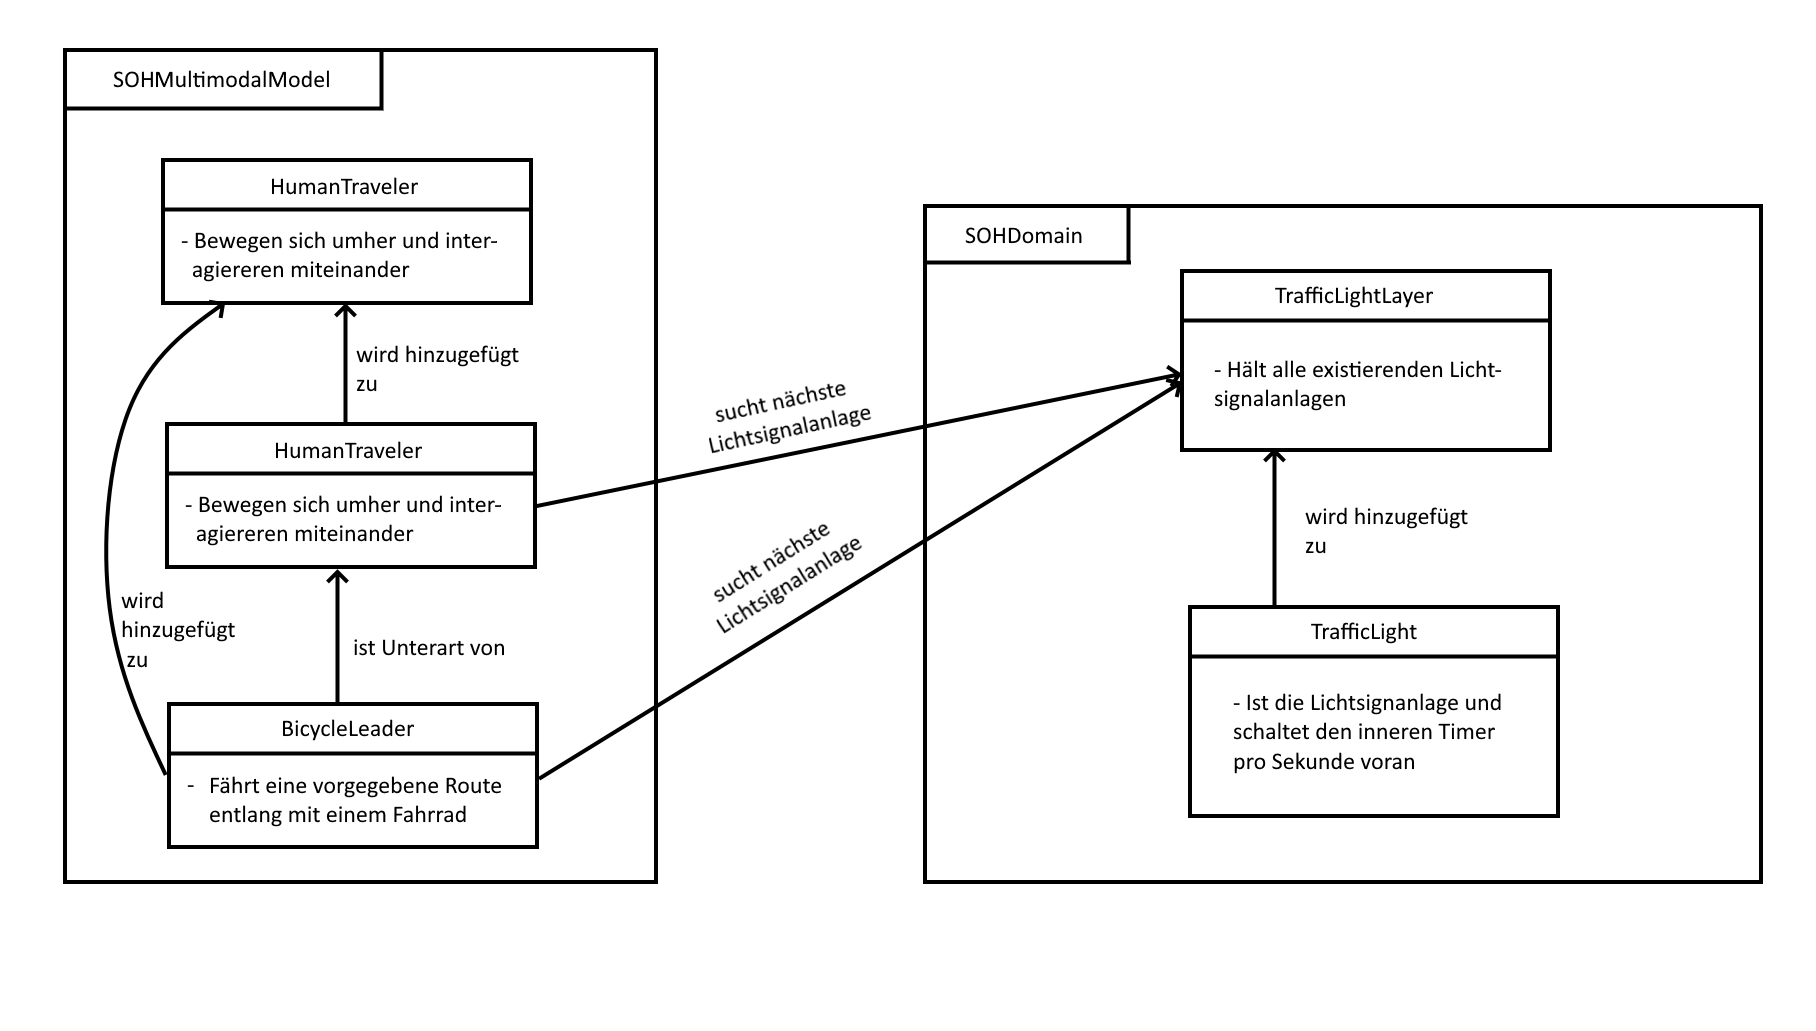
\includegraphics[width=0.75\textwidth]{architecture}
    \caption{Klassendiagramm der Agenten und Entitäten}
    \label{fig:class-diagramm}
\end{figure}

\code{HumanTraveler} werden jede Stunde erschaffen und zu ihrem \code{HumanTravelerLayer} hinzugefügt.
Die erschaffenen \code{HumanTraveler} bewegen sich auf dem \code{HumanTravelerLayer}, auf der sie mit anderen Agenten interagieren können.

Zu jeder vollen Stunde wird ein \code{BicycleLeader} in dem \code{HumanTravelerLayer} hinzugefügt und erhält dann über die \code{BicycleLeaderRoute} die zugewiesenen Routenpunkte, die dieser abfahren muss.

Die \code{TrafficLight}s werden zu Beginn vollständig in die Simulation geladen und zu einem \code{TrafficLightLayer} hinzugefügt.
Danach stehen sie jedem \code{HumanTraveler} zur Verfügung als Referenz, sobald diese wiederum erstellt werden.
\code{BicycleLeader} sind dabei eine Unterklasse der \code{HumanTraveler} und haben somit auch Zugriff auf den \code{TrafficLightLayer}.


Ein \code{TrafficLight} besitzt die folgenden Eigenschaften: Die Position angegeben als \code{Longitude} und \code{Latitude}, eine zufällig zugewiesene GUID namens ,,\code{EntityID}``, die Länge der Rot- und Grünphase als \code{LengthPhaseRed} und \code{LengthPhaseGreen}, die aktuell verstrichene, interne Zeit als \code{CurrTime}, die aktuelle Lichtsignalphase \code{CurrPhase} und zuletzt noch die wartenden Agenten über eine Warteschlange: \code{WaitingRoadUsers}.

\code{HumanTraveler}s können ein \code{Bicycle}, \code{Car} oder nichts bei sich erschaffen.
Eines dieser Modalitäten ist dann ihr Transportmittel, das \code{Vehicle}.

\code{BicycleLeader} sind identisch zu den \code{HumanTraveler}s, bis auf die Einschränkung, dass sie nur \code{Bicycle} nutzen beziehungsweise zu Fuß zum \code{Bicycle} gehen können.


\code{HumanTraveler} nutzen für das Erreichen ihres Zieles den \code{RouteFinder}, mit der sie eine Route zum Abfahren berechnet bekommen.


\code{TrafficLight}s haben folgende Funktionen, die eine Relevanz für sie selbst oder für andere Agenten in der Simulation haben:

\code{public void Tick()} setzt die innere Zeitschaltung der Ampel fort und damit auch die nächste \code{CarLightSignalPhase}, zum Beispiel von Gelb zu Rot.

\code{public void CheckQueue()} überprüft die aktuelle Warteschlange und entfernt, sobald der Agent nicht mehr warten sollte, ihn aus der Warteschlange.

\code{public Boolean Enter(IAgent IAgent)} fügt den angegebenen Agenten zur Warteschlange hinzu, sollte die aktuelle \code{CarLightSignalPhase} Rot sein.

\code{public Boolean CanPass(IAgent IAgent)} gibt einen Wahrheitswert zurück, ob der Agent sich überhaupt in der Nähe der Ampel befindet und wenn ja, ob dieser einfach vorbeifahren kann wegen eines grünen Lichtsignales und keinen wartenden, anderen Agenten.

\code{public Boolean IsQueued(IAgent IAgent)} überprüft und gibt einen Wahrheitswert zurück, ob der Agent noch in der Warteschlange notiert ist.


% The section about the approach of this project on how to determine
% @author Kalvin Döge
%


\section{Herangehensweise zur Ergebnisermittlung}\label{sec:delimitation}

Um

% The section about the projects limits
% @author Kalvin Döge
%


\section{Umfang der Arbeit}\label{sec:delimitation}

Dieser Abschnitt beschäftigt sich mit den Grenzen dieser Arbeit und Simulation.

Dadurch, dass im realen Leben Lichtsignalschaltungen verschiedenster Sicherheitsvorkehrungen unterliegen müssen, damit im Verkehr Sicherheit für alle Verkehrsteilnehmer gewährleistet werden kann, wäre eine Einbindung dieser Vorkehrungen für die Simulation ein wichtiger Realitätsaspekt.
Doch aufgrund von fehlenden Daten und genauer Auskunft der Stadt Hamburg, welche Entscheidungen Lichtsignalanlagen treffen beziehungsweise nach welchem Design sie entwickelt wurden, um die Sicherheit zu ermöglichen, fällt auch dieser Realitätsaspekt aus der Simulation aus.

Zudem werden viele Umwelteinflüsse nicht erst in der Simulation eingebaut: Beispielsweise werden Ereignisse wie Wetter, Unfälle, Baustellen oder verschiedene Verkehrsteilnehmertypen, etwa wie zu langsam Fahrende oder stetig die Spur wechselnde Teilnehmer, nicht berücksichtigt.

Die für diese Simulation genutzten Werte, wie zum Beispiel die der gesamten Agentenzahl oder die der Lichtsignalphasenlänge, sind ebenfalls aufgrund fehlender Statistiken oder Daten nicht sehr realitätsnah.
Beispielsweise wäre es angemessener, jede Lichtsignalschaltung auf der für \code{BicycleLeader} vorgesehenen Route mehrere hunderte Male zu beobachten, nur um dann eine aussagekräftigere Zeit von Rot- und Grünphasen tätigen zu können, damit statistische Abweichungen nicht potenziell das Endergebnis beeinflussen könnten.

Die Realität müsste für die Simulation über die Daten, Umwelteinflüssen und Agententypen abgebildet werden, damit ein praktischer Nutzen für die Stadt Hamburg entstehen könnte.
Entsprechend bleibt der Nutzen dieser Arbeit für die Stadt Hamburg im theoretischen Bereich.

